\documentclass[../main.tex]{subfiles}

\begin{document}

A continuación se muestran los resultados obtenidos tras finalizar el proceso de desarrollo junto a los principales problemas que han surgido para lograr los objetivos y las soluciones propuestas.

\section{Resultados obtenidos}

Tras el desarrollo del proyecto se han obtenido varios resultados, que en su conjunto pueden definirse como un sistema de generación procedimental de laberintos parcialmente no euclidianos que se generan en base al espacio de trabajo disponible por el usuario.

El primer resultado obtenido es la estructura de datos que permite almacenar el laberinto en forma de grafo. Esta parte es la base de todo el resto de resultados conseguidos ya que gracias a que dicha estructura de datos permite tanto almacenar toda la información necesaria como renderizar cualquier sección a partir de sus características, el resto del desarrollo es más simple.

Utilizándola se crea el que es el resultado principal del proyecto, el sistema de generación procedimental. Este sistema, a partir de las características del espacio de trabajo disponible por el usuario, crea laberintos diferentes y completamente aleatorios, cuya longitud puede ser definida. 

El laberinto está formado por diferentes secciones interconectadas entre ellas por portales que hacen que para el usuario parezca que están contiguas unas con otras. Las características de todas las secciones del laberinto así como los portales que las conectan se crean y se almacenan en el grafo antes de renderizar la primera sección, siendo las secciones los nodos y los portales las conexiones entre ellos. Esto significa que lo primero que se hace es generar el laberinto, almacenarlo en la estructura de datos, y más tarde se utiliza para renderizar las secciones necesarias y conectarlas. 

La forma y longitud de las secciones dependen del punto del espacio de trabajo en el que se encuentra el usuario, y dentro de los límites que esto suponga son aleatorias. Además, para que el recorrido sea un laberinto como tal, es necesario que las secciones puedan crear ramificaciones o bifurcaciones en el camino, de manera que no haya un camino único y el usuario pueda perderse. 

La probabilidad de que esto ocurra y la longitud de estos nuevos caminos es algo que se debe tener en cuenta, ya que nuevas ramificaciones en el laberinto pueden crear otras ramificaciones, y así sucesivamente. Si se crean demasiadas ramificaciones podría suponer una dificultad demasiado alta para encontrar el final del laberinto, mientras que si se crean muy pocas, más que un laberinto podría ser un único camino.

Un ejemplo puede verse en la figura \ref{fig:Gameplay_Example}, donde se puede apreciar a la izquierda la escena de Unity, con las secciones renderizadas actualmente, y a la derecha el punto de vista del usuario. Las coordenadas del espacio de trabajo  de $8m^2$ en las que se comienza son (1,1), por lo que la primera sección es un giro a la derecha. Como tiene longitud suficiente, en este caso la sección es en forma de F y se ha creado una nueva ramificación, por lo que la sección tiene 2 pasillos laterales.

\begin{figure}[h!]
\hspace{-1cm}
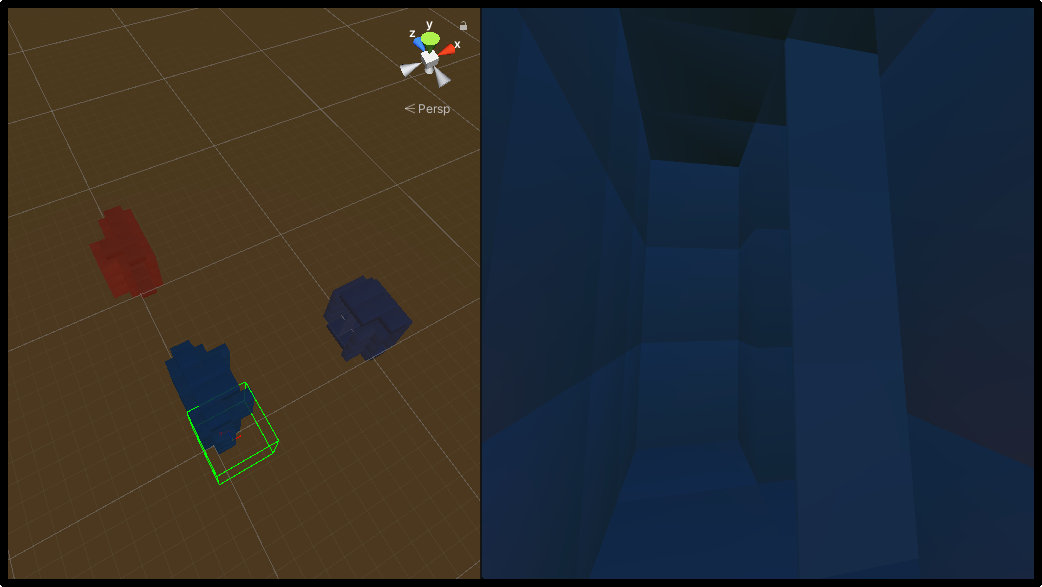
\includegraphics[width=14cm,height=8.5cm]{imagenes/Gameplay_Example.png}
\caption{Situación inicial cuando la primera sección es en forma de F.}
\label{fig:Gameplay_Example}
\end{figure}

Como se explica durante el desarrollo, la elección de qué pasillo lleva por el camino principal y qué pasillo lleva a la nueva ramificación es completamente aleatoria, y las secciones que se generan lo hacen en base a esta decisión. En este caso, como se aprecia en la figura \ref{fig:Both_Hallways}, el primer pasillo lleva por el camino principal, mientras que el segundo pasillo lleva a la nueva ramificación.

Por lo tanto si el usuario decide tomar el primer camino estaría más cerca de llegar al final del laberinto, e iría a otra sección en forma de F, que esta vez gira a la izquierda, donde tendría que tomar otra decisión igual. 

Sin embargo, si decide tomar el segundo camino, entraría a la nueva ramificación, lo que hace que se aleje del objetivo. Si sigue avanzando, dependiendo del número de ramificaciones que tenga el laberinto, al usuario se le hará más difícil volver al camino principal que lleva a la victoria.

Aunque aparentemente las secciones están contiguas, en la escena puede verse que realmente esto no es así. Esto permite generar entornos que de otra manera no serían posibles y crear laberintos de longitud infinita, dado que las secciones de este no se superponen en ninguna situación. Esto último es posible gracias a que en Unity solo se cargan las secciones necesarias en cada momento, aumentando la eficiencia, por lo que una vez calculadas las características de todas las secciones, el número de estas es irrelevante en cuanto a rendimiento.

%%Imagen donde salgan ambos portales y caminos
\begin{figure}[h!]
\hspace{-1cm}
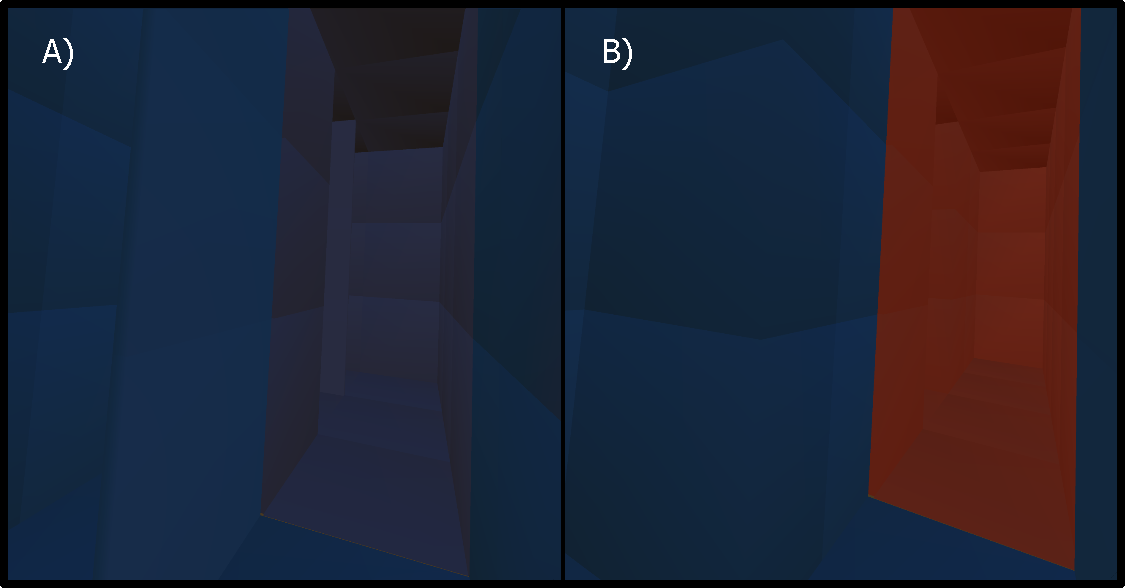
\includegraphics[width=14cm,height=8.5cm]{imagenes/Both_Hallways.png}
\caption{Punto de vista del usuario de los portales de salida de la sección actual. A) Portal de salida que lleva por el camino principal. B) Portal de salida que lleva a la nueva ramificación.}
\label{fig:Both_Hallways}
\end{figure}

Un ejemplo de este tipo de situaciones imposibles puede verse en la figura \ref{fig:Both_Hallways}. La sección inicial es una sección en forma de F cuyos pasillos laterales están contiguos, sin embargo ambas secciones conectadas a estos pasillos realizan un giro a la izquierda. Si las secciones se encontrasen contiguas en el espacio esto sería imposible ya que se superpondrían, como se puede ver en la figura \ref{fig:Impossible_Space}.

Para el usuario esto hace que la experiencia de recorrer el laberinto sea totalmente diferente de la que se consigue recorriendo un laberinto normal. Si desde la primera sección un usuario observa las secciones conectadas a ambos pasillos laterales, cabría esperar que si decide tomar el primer camino, al girar a la izquierda se toparía con la sección conectada al segundo, pero al avanzar ve que no es así, y en su lugar hay otra sección completamente diferente.

Este efecto de contigüidad en las secciones del laberinto es lo que permite que la longitud del laberinto pueda ser infinita. Aunque el usuario dispone de un espacio de trabajo limitado, este se está reutilizando constantemente para cada sección y, aunque en el espacio real estarían superpuestas, en el espacio virtual no lo están. Por ejemplo, podría crearse un laberinto que siempre girase hacia la derecha, pero siempre pasase por secciones distintas. Para el usuario, esto sería como recorrer una habitación rectangular que tiene más de 4 esquinas.

En resumen, como resultado del proyecto se obtiene no solo una estructura de datos que permite almacenar y manipular el espacio virtual como un grafo, sino también un sistema de generación procedimental que aprovecha esta estructura de datos para generar laberintos de longitudes potencialmente infinitas en espacios de trabajo limitados.

\begin{figure}[h!]
\hspace{-1cm}
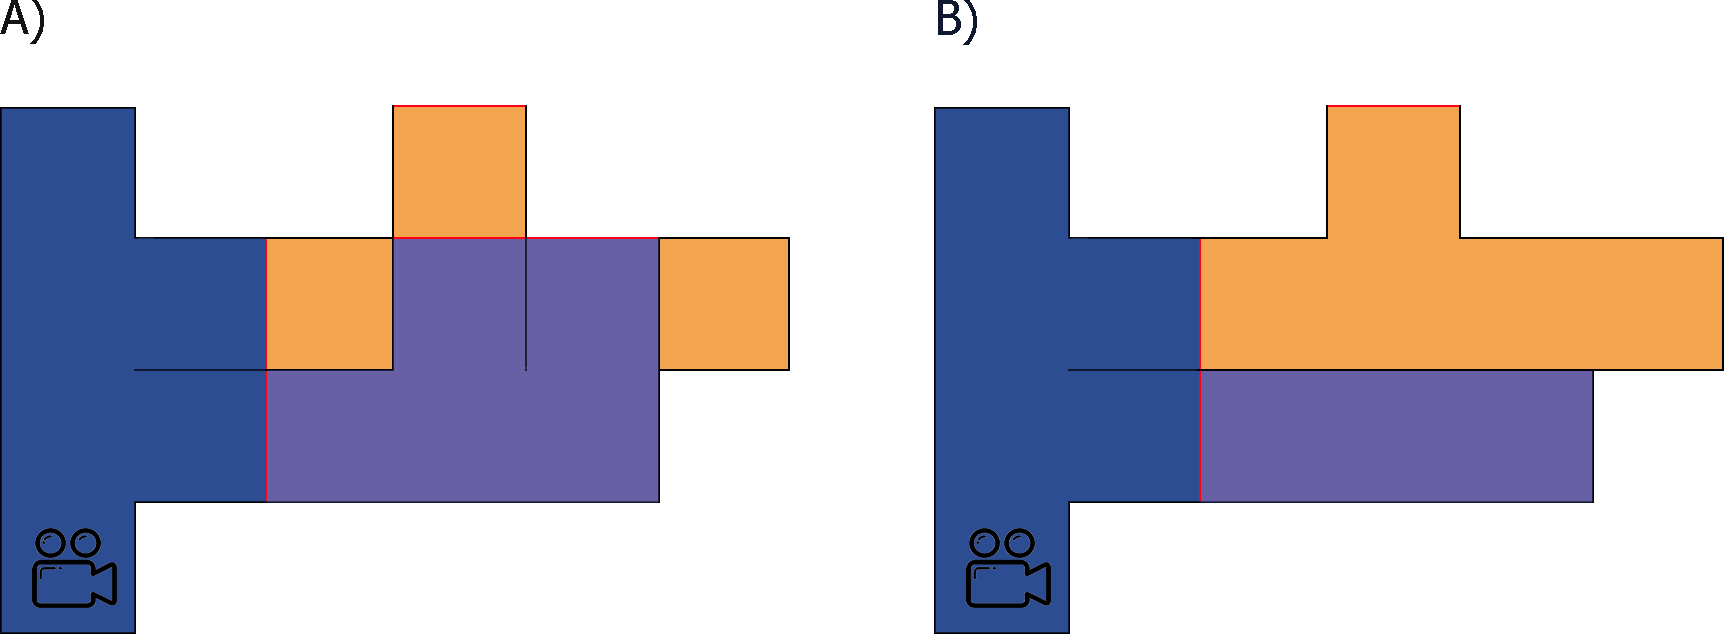
\includegraphics[width=16cm,height=6.5cm]{imagenes/Impossible_Space.png}
\caption{Secciones del laberinto desde el punto de vista de un usuario. A) Sección del camino principal superpuesta. B) Sección de la nueva ramificación superpuesta}
\label{fig:Impossible_Space}
\end{figure}

Adicionalmente, también se consigue un sistema de renderización dinámica cuya finalidad es maximizar el rendimiento en tiempo de ejecución, ya que los portales utilizados en el proyecto suponen una carga computacional considerable. Este sistema renderiza en la escena únicamente las secciones y portales necesarios para que el usuario pueda ver todas las partes posibles del espacio desde la sección en la que se encuentra en determinado momento. En el momento en el que se detecta que el usuario ha cambiado de sección se renderizan y desrenderizan las secciones necesarias para maximizar la eficiencia.

El resultado obtenido permite generar entornos infinitamente grandes en espacios de trabajo limitados haciendo uso de entornos parcialmente no euclidianos, haciendo posible crear entornos virtuales que serían imposibles en el mundo real. Con esto se busca dar una solución al problema del espacio de trabajo mientras se mantiene una sensación de presencia en el entorno virtual lo suficientemente buena como para que el usuario se sienta parte de ella, y no sea necesario preocuparse por el espacio real disponible.

\section{Problemas encontrados}

Durante el desarrollo del proyecto y para cumplir los objetivos y llegar al resultado final se han encontrado varios problemas que ha sido necesario solucionar.

Al trabajar con dispositivos de realidad virtual que cuentan con varias cámaras y multitud de funcionalidades personalizables, durante la migración del efecto de los portales al sistema Unity XR ha sido necesario solucionar problemas de varios tipos. Dado el funcionamiento del teletransporte de los portales, es necesario controlar las cámaras de cada uno de los ojos por separado, pero como el sistema XR no ofrece herramientas para conseguirlo, es necesario hacerlo manualmente en Unity.

También se presentan problemas de rendimiento, ya que este efecto es compu -tacionalmente pesado. Esto supone que la visión del portal quede distorsionada, lo que hace que se pierda la sensación de inmersión en el entorno virtual. Por esto, una vez migrado el efecto, ha sido necesario realizar ajustes y cambios para mejorar el rendimiento y conseguir que la textura que se visualiza en el portal sea prácticamente indistinguible de lo que se vería si las secciones estuviesen contiguas.

Como los laberintos generados tienen múltiples secciones y todas ellas tienen portales para interconectarse, se generan más problemas de rendimiento, dado que cuantos más portales hayan renderizados en la escena, peor funciona. Este problema se ha resuelto con el sistema de renderización dinámica, que asegura que en todo momento están renderizados el menor número de portales posible.

Aunque generar entornos virtuales procedimentalmente añade una variedad casi infinita, también genera muchos problemas. Al estar trabajando con entornos parcialmente no euclidianos y siendo uno de los principales objetivos del proyecto generar el laberinto dentro de los límites del espacio de trabajo del usuario, es necesario controlar las direcciones y características de las secciones relativamente a lo que ve el usuario y no a su situación en la escena de Unity. 

También hay que asegurar que en todo momento el entorno generado no permita que el usuario salga de su espacio de trabajo y, al estar trabajando con este tipo de entornos y laberintos que generan ramificaciones recursivamente de características y longitudes aleatorias, no es trivial asegurar que en todos los casos esto se cumple.

\begin{figure}[h!]
\hspace{-1.25cm}
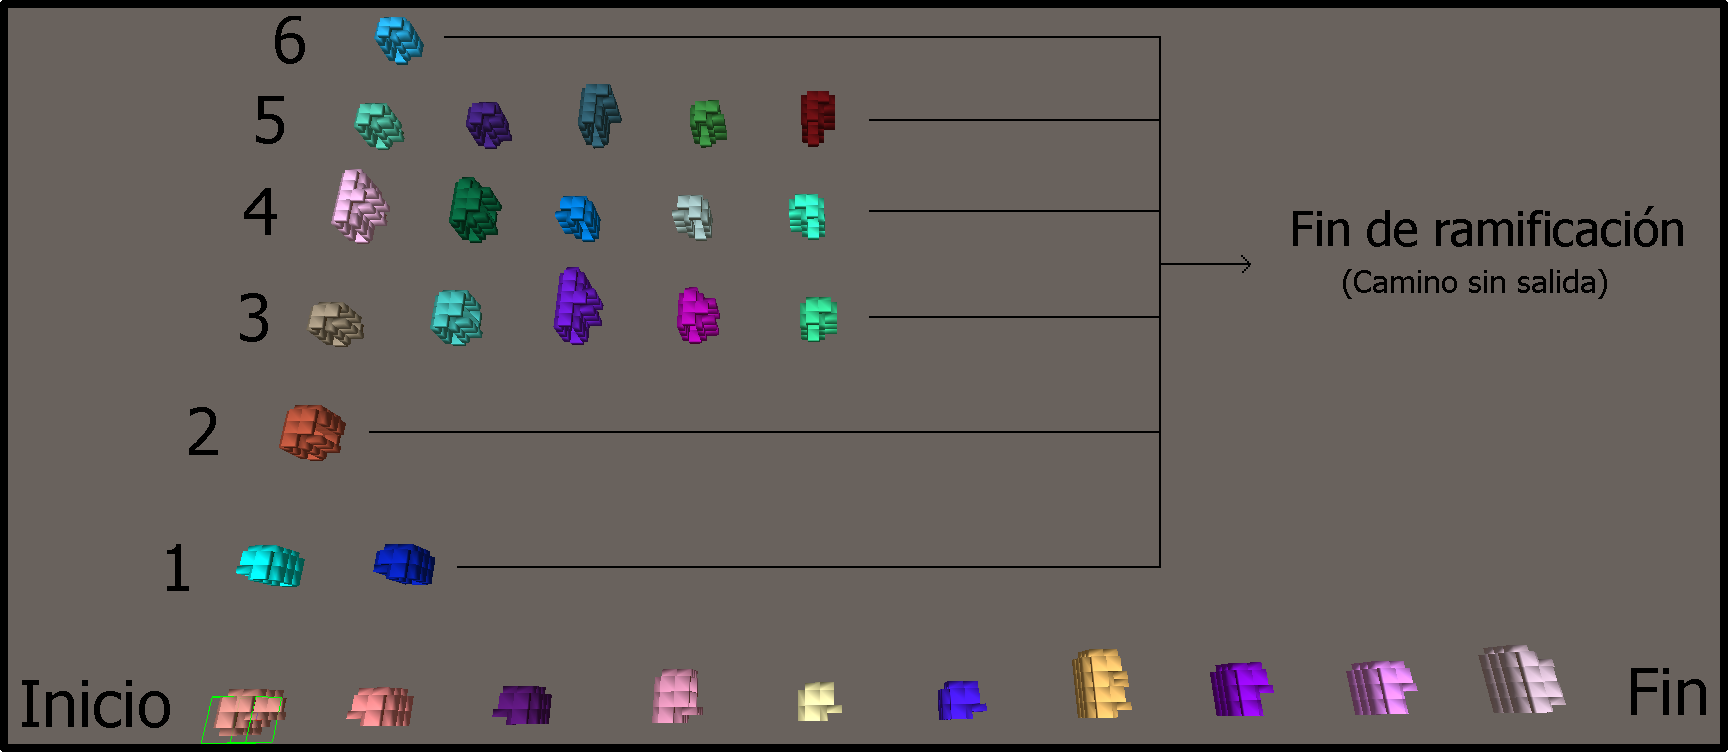
\includegraphics[width=14.5cm,height=7cm]{imagenes/Full_Maze.png}
\caption{Vista vertical de un laberinto renderizado al completo y cuyas ramificaciones y secciones están separadas evitando superposiciones.}
\label{fig:Full_Maze}
\end{figure}

Las secciones deben repartirse por la escena de forma que nunca sea posible que se superpongan unas con otras. Como tanto la longitud del laberinto como el número de ramificaciones son aleatorios, para conseguirlo se separan las ramificaciones en el momento de su generación en filas, y sus secciones se separan horizontalmente lo suficiente como para que en el peor caso sea imposible que colisionen unas con otras. Un ejemplo puede verse en la figura \ref{fig:Full_Maze}, donde se puede observar un laberinto renderizado al completo con 6 ramificaciones distintas separadas en filas, cuyas secciones están separadas horizontalmente.

Además de la renderización del laberinto como conjunto, la renderización de cada sección por separado también genera problemas, ya que al ser sus caracte- rísticas completamente aleatorias hay muchas excepciones y casos que hay que controlar. Un ejemplo son las secciones en forma de F cuyos pasillos laterales están contiguos, siendo necesario minimizar el grosor de la pared que los separa para permitir al usuario ver ambos portales sin problemas. La posición y rotación de los objetos que forman la sección deben ser correctas en todo momento para mantener la sensación del usuario de presencia en el entorno virtual.

En general, trabajar con dispositivos de realidad virtual y el sistema XR que es relativamente nuevo, ha supuesto algunos problemas que ha sido necesario resolver para cumplir con los objetivos del proyecto. Además, trabajar con algoritmos procedimentales añade más dificultad en el desarrollo ya que, al existir infinidad de posibilidades en cada ejecución, es complicado controlar todas y cada una de las excepciones.

\end{document}
